% ------------------------------------------------------------------------
% ------------------------------------------------------------------------
% Modelo de relatório de estágio DAS - UFSC.
% Esse modelo usa abnTeX2 (https://www.abntex.net.br/)
% ------------------------------------------------------------------------
% ------------------------------------------------------------------------

\documentclass[
	% -- opções da classe memoir --
	12pt,				% tamanho da fonte
	openright,			% capítulos começam em pág ímpar (insere página vazia caso preciso)
	oneside,			% Para impressão simples. Para impressão frente e verso, use twoside
	a4paper,			% tamanho do papel. 
	% -- opções do pacote babel --
	english,			% idioma adicional para hifenização
	brazil				% o último idioma é o principal do documento
	]{abntex2}

% ---
% Pacotes básicos 
% ---
\usepackage{lmodern}			% Usa a fonte Latin Modern			
\usepackage[T1]{fontenc}		% Selecao de codigos de fonte.
\usepackage[utf8]{inputenc}		% Codificacao do documento (conversão automática dos acentos)
\usepackage{lastpage}			% Usado pela Ficha catalográfica
\usepackage{indentfirst}		% Indenta o primeiro parágrafo de cada seção.
\usepackage{color}				% Controle das cores
\usepackage{graphicx,float}		% Inclusão de gráficos
\usepackage{microtype} 			% para melhorias de justificação
\usepackage{hyperref}
% ---
		
% ---
% Pacotes de citações
% ---
\usepackage[brazilian,hyperpageref]{backref}	 % Paginas com as citações na bibl
\usepackage[alf]{abntex2cite}	% Citações padrão ABNT

% --- 
% CONFIGURAÇÕES DE PACOTES
% --- 

% ---
% Configurações do pacote backref
% Usado sem a opção hyperpageref de backref
\renewcommand{\backrefpagesname}{Citado na(s) página(s):~}
% Texto padrão antes do número das páginas
\renewcommand{\backref}{}
% Define os textos da citação
\renewcommand*{\backrefalt}[4]{
	\ifcase #1 %
		Nenhuma citação no texto.%
	\or
		Citado na página #2.%
	\else
		Citado #1 vezes nas páginas #2.%
	\fi}%
% ---

% ---
% Informações de dados para CAPA e FOLHA DE ROSTO
% ---
\titulo{Titulo: subtítulo}
\autor{Breno Barroso Moreira}
\local{Florianópolis}
\data{2025}
\orientador{Carlos Barros Montez }
\coorientador{} % Deixar vazio caso não haja
\instituicao{%
  UNIVERSIDADE FEDERAL DE SANTA CATARINA
  \par
  CENTRO TECNOLÓGICO
  \par
  DEPARTAMENTO DE AUTOMAÇÃO E SISTEMAS}
\tipotrabalho{Relatório de Estágio}

\preambulo{Relatório submetido à Universidade Federal de Santa Catarina como requisito para a aprovação na disciplina \textbf{DAS 5501 - Estágio em Controle e Automação Industrial} do curso de Graduação em Engenharia de Controle e Automação.}
% ---

% ---
% Configurações de aparência do PDF final

% alterando o aspecto da cor azul
\definecolor{blue}{RGB}{41,5,195}

% informações do PDF
\makeatletter
\hypersetup{
     	%pagebackref=true,
		pdftitle={\@title}, 
		pdfauthor={\@author},
    	pdfsubject={\imprimirpreambulo},
	    pdfcreator={LaTeX with abnTeX2},
		pdfkeywords={abnt}{latex}{abntex}{abntex2}{trabalho acadêmico}, 
		colorlinks=true,       		% false: boxed links; true: colored links
    	linkcolor=black,          	% color of internal links
    	citecolor=blue,        		% color of links to bibliography
    	filecolor=magenta,      		% color of file links
		urlcolor=blue,
		bookmarksdepth=4
}
\makeatother
% --- 

% --- 
% Espaçamentos entre linhas e parágrafos 
% --- 

% O tamanho do parágrafo é dado por:
\setlength{\parindent}{1.3cm}

% Controle do espaçamento entre um parágrafo e outro:
\setlength{\parskip}{0.2cm}  % tente também \onelineskip

% ---
% compila o indice
% ---
\makeindex
% ---

% ----
% Início do documento
% ----
\begin{document}

% Retira espaço extra obsoleto entre as frases.
\frenchspacing 

% ----------------------------------------------------------
% ELEMENTOS PRÉ-TEXTUAIS
% ----------------------------------------------------------
% \pretextual

% ---
% Capa
% ---

\renewcommand{\imprimircapa}{%
  \begin{capa}%
    \center
    \ABNTEXchapterfont\Large\textbf\imprimirinstituicao
    
    \vspace*{1cm}
    
    {\ABNTEXchapterfont\large\textbf\imprimirautor}
    
    \vfill
    \begin{center}
    \ABNTEXchapterfont\bfseries\ Relatório de Estágio \\
    \ABNTEXchapterfont\bfseries\LARGE\imprimirtitulo
    \end{center}
    \vfill
    
    \large\imprimirlocal
    
    \large\imprimirdata
    
    \vspace*{1cm}
  \end{capa}
}

\imprimircapa
% ---

% ---
% Folha de rosto
% (o * indica que haverá a ficha bibliográfica)
% ---
\makeatletter
\renewcommand{\folhaderostocontent}{
  \begin{center}
  
    {\ABNTEXchapterfont\large\textbf\imprimirautor}
    
    \vspace*{\fill}\vspace*{\fill}
    
    \begin{center}
    	\ABNTEXchapterfont\bfseries\Large\imprimirtitulo
    \end{center}
    
    \vspace*{\fill}
    
    \abntex@ifnotempty{\imprimirpreambulo}{%
      \hspace{.45\textwidth}
      \begin{minipage}{.5\textwidth}
      \SingleSpacing
      \imprimirpreambulo
      \par
      {\imprimirorientadorRotulo~\imprimirorientador\par}
      \abntex@ifnotempty{\imprimircoorientador}{%
    	{\imprimircoorientadorRotulo~\imprimircoorientador}%
      }%
      \end{minipage}%
      \vspace*{\fill}
    }%
    
    \vspace*{\fill}
    
    {\large\imprimirlocal}
    
    \par
    
    {\large\imprimirdata}
    
    \vspace*{1cm}
  \end{center}
}
\makeatother

\imprimirfolhaderosto
% ---

% ---
% Inserir folha de aprovação
% ---

% Isto é um exemplo de Folha de aprovação, elemento obrigatório da NBR
% 14724/2011 (seção 4.2.1.3). Você pode utilizar este modelo até a aprovação
% do trabalho. Após isso, substitua todo o conteúdo deste arquivo por uma
% imagem da página assinada pela banca com o comando abaixo:
%
% \includepdf{folhadeaprovacao_final.pdf}
%
\makeatletter
\begin{folhadeaprovacao}

  \begin{center}
    {\ABNTEXchapterfont\large\imprimirautor}

    \vspace*{\fill}\vspace*{\fill}
    \begin{center}
      \ABNTEXchapterfont\bfseries\Large\imprimirtitulo
    \end{center}
    \vspace*{\fill}
    
    Este relatório de estágio foi julgado no contexto da disciplina DAS5501: Estágio em Controle e Automação Industrial e \textbf{APROVADO} na sua forma final pelo Curso de Engenharia de Controle e Automação.
    
    \vspace*{\fill}
    
    Florianópolis, \today
  \end{center}
  
   \assinatura{\textbf{\imprimirorientador} \\ Orientador \\ Universidade Federal de Santa Catarina}
   
   \assinatura{\textbf{Marcia Medina} \\ Supervisor na Empresa \\ EMPRESA}
      
   \abntex@ifnotempty{\imprimircoorientador}{%
     \assinatura{\textbf{\imprimircoorientador} \\ Co-orientador \\ Universidade Federal de Santa Catarina}
   }%
\makeatother
   
        
\end{folhadeaprovacao}
% ---

% ---
% Dedicatória
% ---
\begin{dedicatoria}
   \vspace*{\fill}
   \centering
   \noindent
   \textit{Dedicatória: OPCIONAL} \vspace*{\fill}
\end{dedicatoria}
% ---

% ---
% Agradecimentos
% ---
\begin{agradecimentos}
(OPCIONAL): Essa seção não possui uma estrutura pré-definida. O mais usual é separar em parágrafos. Mencionar apenas pessoas, instituições e outros que tenham tido importância para a realização do trabalho.

\end{agradecimentos}
% ---

% ---
% Epígrafe
% ---
\begin{epigrafe}
    \vspace*{\fill}
	\begin{flushright}
		\textit{``Epígrafe (Opcional – NBR10520). Elemento opcional, no qual o autor apresenta uma citação, seguida de indicação de autoria, relacionada à matéria tratada no corpo do trabalho.''}
	\end{flushright}
\end{epigrafe}
% ---

% ---
% RESUMOS
% ---

% resumo em português
\setlength{\absparsep}{18pt} % ajusta o espaçamento dos parágrafos do resumo
\begin{resumo}
	 Apresenta as informações principais do documento (Descrição geral da empresa (natureza, mercado, processos, etc.), problema-foco atacado no PFC, o que foi feito, principais resultados atingidos, etc.). Deve conter entre 100 e 500 palavras (NBR 6028/2003) em um único parágrafo. Se o documento for escrito em outra língua que não o Português, então é necessário fazer um Resumo \textbf{Estendido} em Português, ao invés deste resumo enxuto.

\vspace{\onelineskip}

\noindent 

\textbf{Palavras-chave:} No mínimo 3 (três) e separadas por ponto (.) 
\end{resumo}

% resumo em inglês
\begin{resumo}[Abstract]
 \begin{otherlanguage*}{english}
	Resumo em língua inglesa. Mesma formatação do Resumo.

\vspace{\onelineskip}

\noindent 
\textbf{Key-words}: No mínimo 3 (três) e separadas por ponto (.) 
 \end{otherlanguage*}
\end{resumo}

% Inserir listas. Todas essas listas são opcionais.
% ---
% inserir lista de ilustrações
% ---
\pdfbookmark[0]{\listfigurename}{lof}
\listoffigures*
OPCIONAL
\cleardoublepage
% ---

% ---
% inserir lista de tabelas
% ---
\pdfbookmark[0]{\listtablename}{lot}
\listoftables*
OPCIONAL
\cleardoublepage
% ---

% ---
% inserir lista de abreviaturas e siglas
% ---
\begin{siglas}
  \item[ETL] Extract, Transform and Load
\end{siglas}
% ---

% ---
% inserir lista de símbolos
% ---
\begin{simbolos}
  \item[$ \Gamma $] OPCIONAL
\end{simbolos}
% ---


% ---
% inserir o sumario
% ---
\pdfbookmark[0]{\contentsname}{toc}
\tableofcontents*
\cleardoublepage
% ---



% ----------------------------------------------------------
% ELEMENTOS TEXTUAIS
% ----------------------------------------------------------
\textual

% Desenvolvimento
\chapter{Introdução}

O presente trabalho detalha as atividades desenvolvidas durante o estágio obrigatório na empresa LifesHub, em Florianópolis, no ano de 2025, focadas no desenvolvimento de um sistema de processamento de dados para o setor de saúde suplementar. O trabalho aborda a criação de um pipeline de Extração, Transformação e Carga (ETL), projetado para automatizar a coleta, o tratamento e o enriquecimento de grandes volumes de dados públicos. O problema central que norteia este projeto é a alta complexidade e a descentralização das fontes de dados de saúde no Brasil, um obstáculo que dificulta a geração de análises estratégicas e inteligência de mercado para os agentes do setor.

\section{Contextualização}

O cenário da saúde suplementar no Brasil é caracterizado por um ecossistema de dados vasto e diversificado, disponibilizado publicamente por diferentes órgãos governamentais. Fontes como a ANS, CNES e o DATASUS (com seus subsistemas SIH, SIA e CIHA) oferecem um volume massivo de informações sobre operadoras, beneficiários, estabelecimentos e procedimentos. No entanto, a extração de valor desses dados é um desafio significativo. As informações são descentralizadas, armazenadas em formatos heterogêneos — como arquivos de banco de dados (.dbc), planilhas (.xlsx) e texto (.csv) — e frequentemente exigem um complexo processo de limpeza, padronização e cruzamento para se tornarem úteis.

Nesse contexto, a LifesHub se posiciona como uma empresa de tecnologia especializada em resolver essa complexidade. A companhia atua na consolidação e no enriquecimento desses dados públicos, transformando-os em uma plataforma de inteligência de mercado para os diversos players do setor, como hospitais, operadoras de planos de saúde e indústria farmacêutica. O projeto desenvolvido neste estágio está diretamente inserido nessa missão, focando na construção da infraestrutura de engenharia de dados — o pipeline de ETL — responsável por automatizar e escalar a capacidade da empresa de processar e entregar dados de alta qualidade.
A arquitetura desta solução e as tecnologias empregadas serão detalhadas nos capítulos subsequentes.

\newpage
\section{Contexto na Engenharia de Controle e Automação}

O desenvolvimento deste projeto aplica diretamente os conceitos fundamentais da Engenharia de Controle e Automação, indo além de um simples processamento de dados para construir um sistema verdadeiramente autônomo. As conexões com a área são evidentes nos seguintes pilares:

\textbf{Automação e Controle Supervisório:} 

O sistema implementa um controle em malha aberta com supervisão automatizada. Um agente de software (bot) monitora continuamente as fontes de dados externas, como servidores FTP Ao identificar um evento, ele dispara a execução do pipeline de ETL correspondente, funcionando como um controlador que automatiza todo o fluxo de trabalho sem intervenção humana.

\textbf{Integração de Sistemas:}

O projeto é um caso prático de integração de sistemas. A solução orquestra a comunicação entre tecnologias distintas, incluindo servidores FTP, a plataforma de armazenamento em nuvem Azure Blob Storage e o motor de processamento em memória DuckDB.

\textbf{Programação e Desenvolvimento de Sistemas:}

A implementação da lógica foi realizada em Python, seguindo uma arquitetura modular com responsabilidades bem definidas entre orquestração, execução e configuração, aplicando os princípios de desenvolvimento de sistemas automatizados.

\textbf{Análise de Dados para Otimização:}

O objetivo final do sistema automatizado é fornecer dados consistentes e atualizados que sirvam de base para a tomada de decisão estratégica. Ao garantir a disponibilidade de informações de alta qualidade, o projeto habilita a aplicação de técnicas de avaliação de desempenho, essencial para a otimização de processos no setor de saúde.

\section{Objetivos}

O principal objetivo deste projeto é o desenvolvimento de um pipeline de Etração, Transformação e Carga de dados. Os requisitos para que seja alcançado um bom resultado, é a robustez, escabilidade e automação do processo, focando no processamento de dados do setor de saúde suplementar no Brasil. A solução procura converter um grande volumes de dados públicos brutos, vindos de diferentes fontes em um ativo de dados estruturado e confiável e pronto para análise. Todo o sistema foi desenhado para garantir armazenamento e acessibilidade dos dados, agregando valor para os clientes da empresa.

Adicionalmente, era necessário que o sistema fosse escálavel e flexível, empregando tecnologias open-source como Python e DuckDB, integradas a infraestrutura de nuvem da Microsoft Azure. Toda a soluçaõ foi modularizada e configuarada, facilitando a implantação, manutenção e futuras modificações. Esta estrutura garante que o sistema possa ser estendida para novos casos de usos ou novas fontes de dados.

Foram definidos os seguintes objetivos:

\begin{itemize}
    \item Orquestrador de pipelines modular em Python para gerenciar a execução das tarefas, garantindo automação do fluxo de dados.
    \item Implementar o DuckDB como processamento analítico para gerenciar e transformar os dados brutos.
    \item Utilizar o sistema de Azure para servir como repositório centralizado. Armazenamento de dados brutos e processados.
\end{itemize}

\section{Metodologia}

Essa seção descreve as metodologias e princípios utilizados durante a realização do estágio na empresa. Essas práticas garantem uma colaboração organizada entre os os colaboradores durante diferentes fases de desenvolvimento.

\subsection{Framework Scrum}

Aplicamos a metodolgia ágil de gerenciamento de projetos SCRUM. Com ciclos curtos chamados sprints, entregamos valor de forma continua e adáptavel. As cerimônias foram adaptadas ao ritmo da equipe da seguinte forma.

\textbf{Planejamento e execução:} O trabalho foi organizado em ciclos de duas semanas. As tarefas desenvolvidas eram selecionadas através do backlog e movidas para a sprint no início de cada ciclo.

\textbf{Reuniões:} Todas as terças-feiras, a equipe realizava a weekly, para discutirmos o progresso das tarefas em andamentos, identificar impedintos e alinhas as prioridades para o resto da semana.

\textbf{Gerenciamento de tarefas e documentação:} A ferramenta Notion foi utilizada como plataforma de controle. Nela, eram mantidos os quadros de tarefas (cards), o backlog, e o registro de horas (log de horas) dedicado a cada atividade, garantindo o acompanhamento detalhado do processo de cada entrega.

\subsection{Versionamento de código}

O controle de versão do código-fonte do projeto foi realizado através do Git. A escolha dessa ferramenta foi fundamental para permitir o desenvolvimento paralelo de novas funcionalidades, correção de bugs de forma isolada e colaboração entre membros da equipe sem o risco de sobrescrever o trabalho.

A estratégia de ramificação, branching, permitiu o controle de novas implentações de forma contínua, após validades integradas ao código principal (main). Assim, garantindo estabilidade e integridade ao sistema.

\begin{figure}[H]
  \centering
  \caption{Git workflow}\label{fig:git_workflow}
  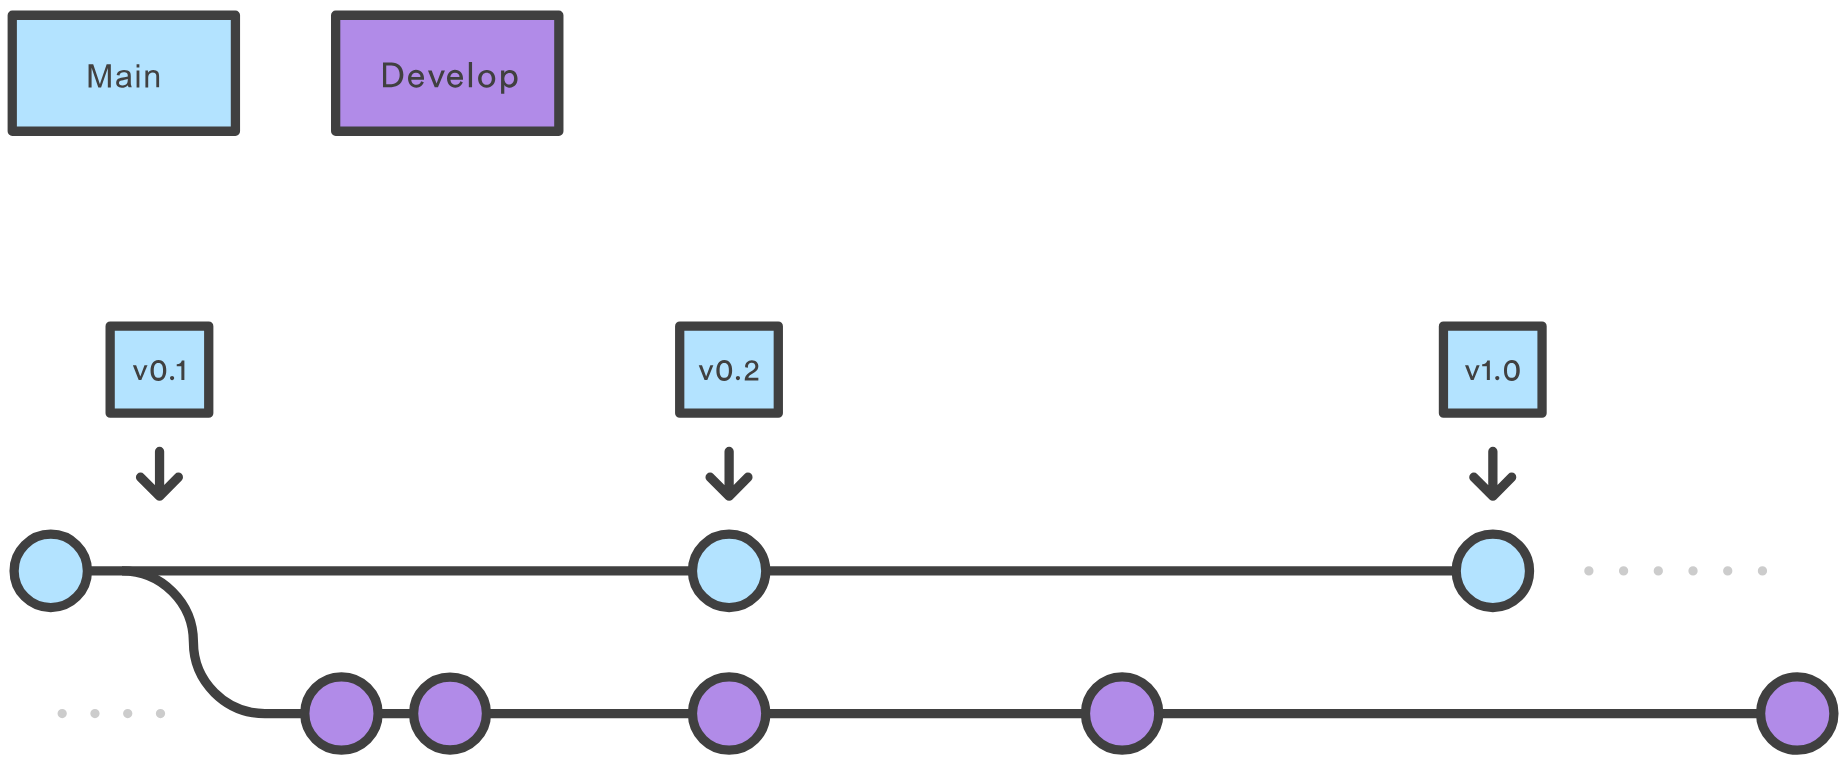
\includegraphics[width=.6\linewidth]{imagens/gitflow.png}
  \par
  \footnotesize{Fonte:TROCAR.}
\end{figure}

\section{Estrutura do documento}

\begin{itemize}
    \item \textbf{Capítulo 2 -- A empresa:} Esse Capítulo introduz a empresa e o processo organizacional.
    \item \textbf{Capítulo 3 -- Fundamentação teórica:} Esse Capítulo traz os fundamentos das teorias, conceitos e tecnologias utilizados durante o projeto.
    \item \textbf{Capítulo 4 -- Arquitetura e requisitos:} Esse Capítulo traz toda arquitetura e componentes da base do projeto. Assim como, os requisitos para a validação.
    \item \textbf{Capítulo 5 -- Desenvolvimento:} Esse Capítulo traz toda a estruturação do problema, e o desenvolvimento de análises, explicando o por quê de cada escolha durante o projeto.
    \item \textbf{Capítulo 6 -- Resultados e análises:} Esse Capítulo valida os passos tomados para garantir o sucesso do projeto. 
    \item \textbf{Capítulo 7 -- Conclusão e trabalhos futuros:} Esse Capítulo recapitula todos os processos e traz sugestões para novas funcionalidades do projeto.
\end{itemize}

\chapter{Capítulo 2}

Descrição da empresa, processos, layouts, problemas, indicadores existentes, etc.

No Capítulo 2, deve-se fazer uma descrição da empresa, processos, layouts, problemas, etc., ou seja, mais detalhadamente motivar e enquadrar o problema dentro do que proporão (a ser descrito no próximo capítulo).

\chapter{Fundamentação teórica}

Este capítulo cobre toda os conceitos fundamentais e teorias necessárias para compreender o projeto apresentando nesse documento.

\section{Processos de ETL}

O ETL é uma sigla para o processo de Extração, Transformação e Carregamento (do inglês extract -transform - load). Ele é uma integração de dados composta por três etapas de tratamentos de dados. Responsável por consilidar os dados em um repositório centralizado, chamado de Data Warehouse, e otimizado para análise. Podemos conferir seu processo descrito abaixo e graficamente através da Figura\ref{fig:etl_process}. \cite{ucommerce_etl}

\begin{itemize}
    \item \textbf{Extração:} Sua primeira fase se trata da coleta de dados brutos das fontes originais. A partir disso, os dados são extraídos para um único formato.
    \item \textbf{Transformação:} Em segundo lugar, a etapa de transformar envolve a limpeza dos dados. Onde os dados extraídos são tratados, padronizados e eliminam os erros e inconsistências dos arquivos originais. Assim, podendo serem analisados.
    \item \textbf{Carregamento:} Após os tratamentos dos dados, podemos partir para o carregamento. Nessa fase, os dados são transmitidos realizando a carga de dados no Data Warehouse.
\end{itemize}

\begin{figure}[H]
  \centering
  \caption{Processo de ETL}\label{fig:etl_process}
  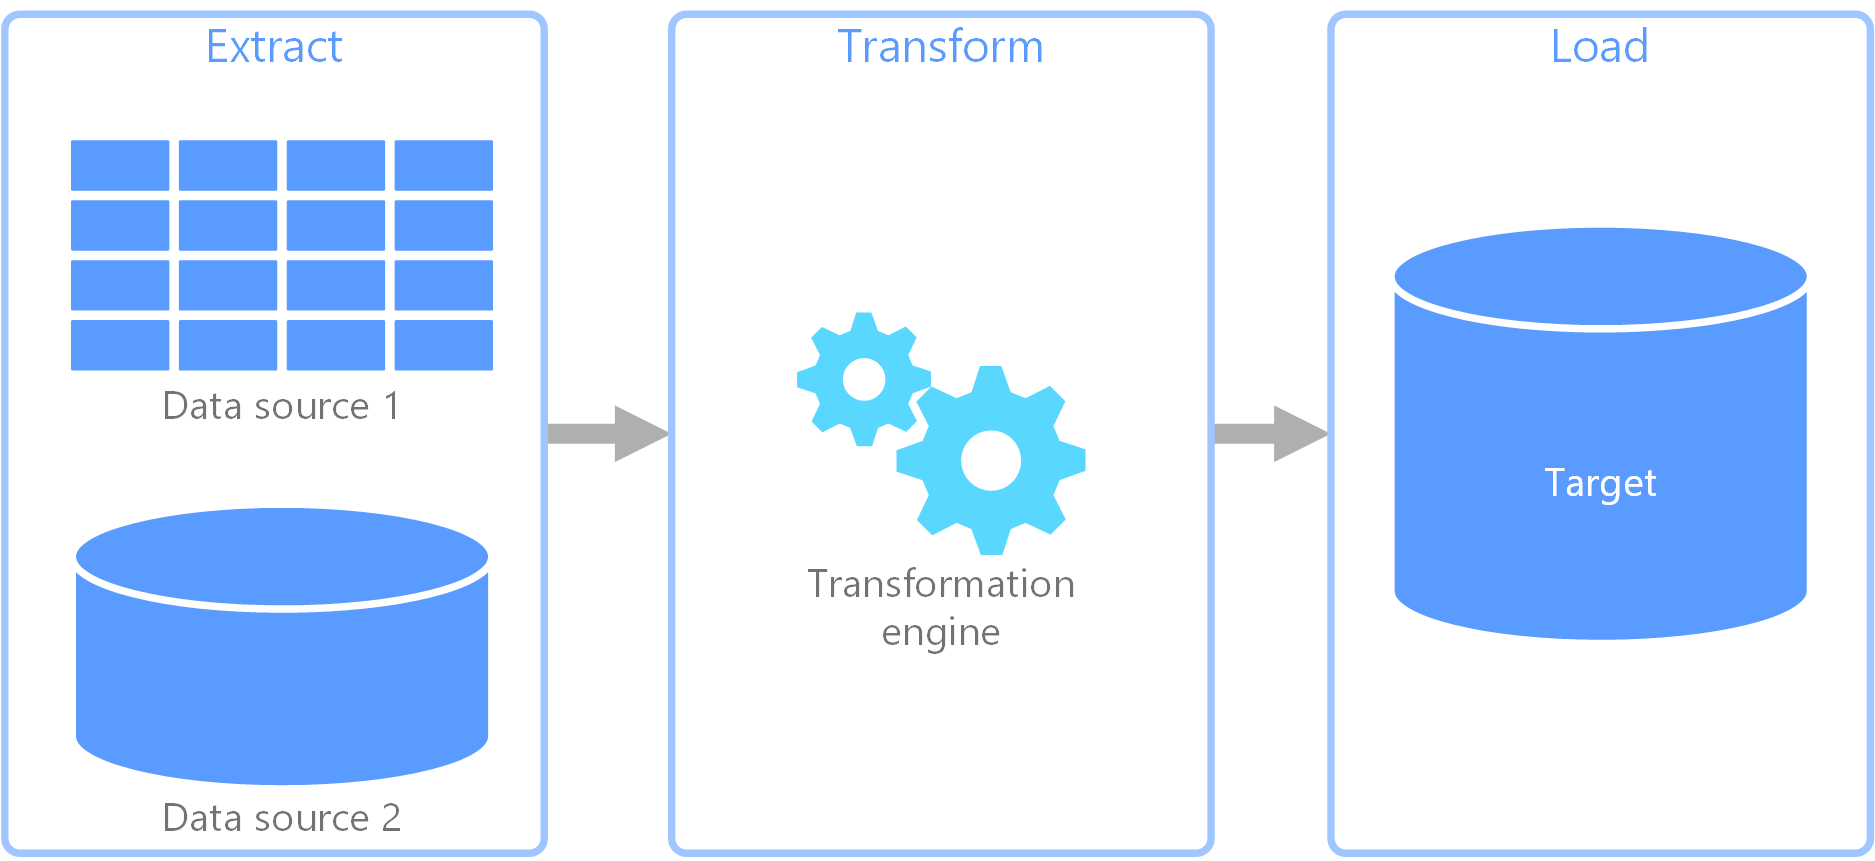
\includegraphics[width=.6\linewidth]{imagens/etl.png}
  \par
  \footnotesize{Fonte:\cite{microsoft_etl}.}
\end{figure}

\subsection{Data Warehouse}

Um data warehouse se trata de um repositório centralizado que contenha todos dados atualizados e necessários para uma organização.

Os dados são importados de diversos tipos de fontes e servem para agregar dados brutos (desestruturados) tanto quanto dados processados (estruturados) através do processo de ETL.\cite{talent500_dwdm}

Analistas de negócios, engenheiros de dados, cientistas de dados e tomadores de decisões acessam os dados por meio de ferramentas de business intelligence (BI), clientes SQL e outras aplicações de análise.

\begin{figure}[H]
  \centering
  \caption{Arquitetura de um Data Warehouse}\label{fig:datawarehouse}
  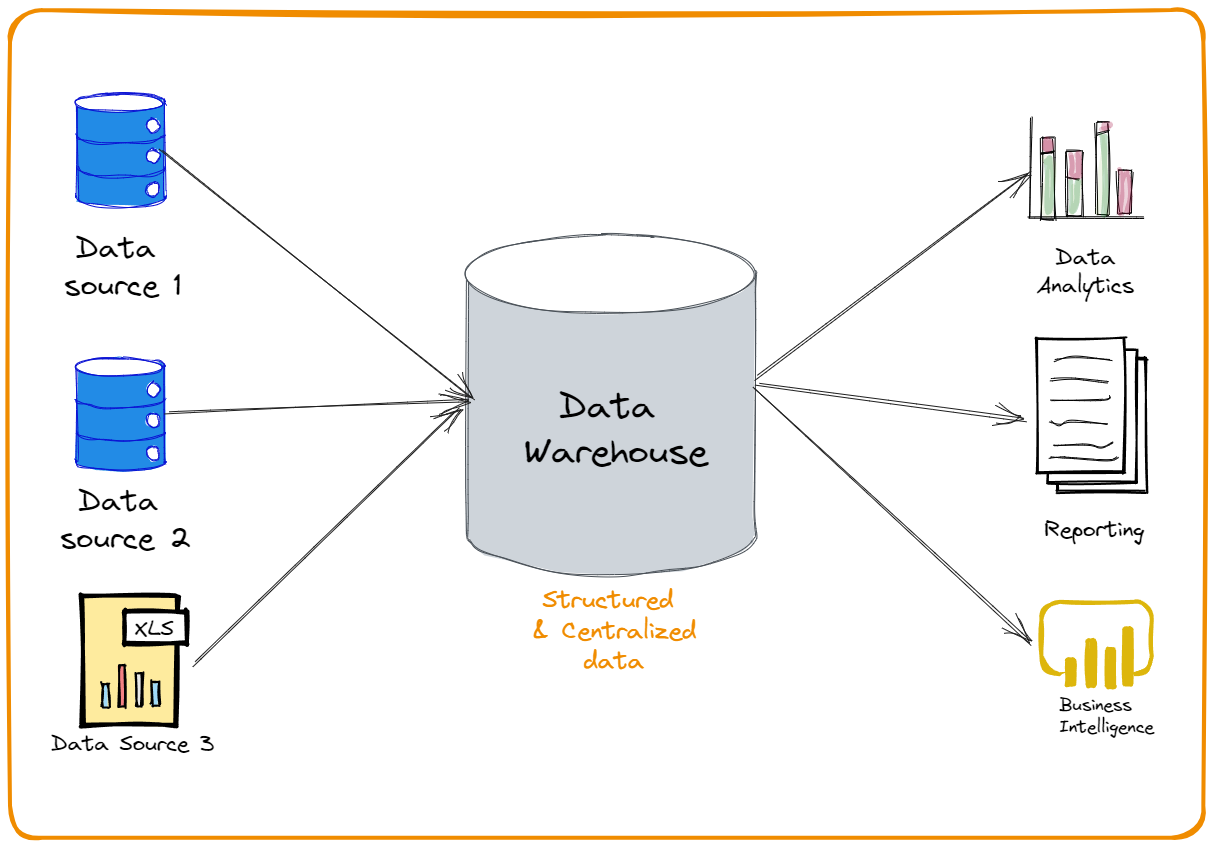
\includegraphics[width=.6\linewidth]{imagens/datawarehouse.png}
  \par
  \footnotesize{Fonte:\cite{aws_dwh}}
\end{figure}

\section{Ferramentas utilizadas para o desenvolvimento}
\subsection{Visual Studio Code}

O Visual Studio Code é um editor de código-fonte leve, mas poderoso, que é executado na área de trabalho e está disponível para Windows, macOS e Linux. Ele vem com suporte integrado para JavaScript, TypeScript e Node.js, além de um rico ecossistema de extensões para outras linguagens e ambientes de execução (como C++, C\#, Java, Python, PHP, Go, .NET).\cite{microsoft_vs}

Além disso, é possível integrar a IDE com ferramentas como debuugers, IAs e verisonamento de controle de código, aumentando a produtividade do processo de desenvolvimento.

\subsection{Python}

Python é uma linguagem de alto nivel versátil, comumente usando no contexto da engenharia de dados. Posusi uma sintaxe simples e legível, tornando acessível para iniciantes e poderosa para usuários avançados. A linguagem oferece um grande ecossistema de librarys (pacotes), como DuckDB, azure-storage-blob, PyYAML, entre outros, essenciais para o projeto. Esses pacotes provém robustez para manipulação de dados, a base do trabalho que está sendo tratado. Além disso, a facilidade da integração de outros tipos de arquivos, como JSON, YML, CSV, Excel e bancos de dados é um diferencial da linguagem. Diante dessas características, Python foi a melhor escolha para atuar como orquestrador central do pipeline de ETL.\cite{python_about}

\subsection{Package: azure-storage-blob}

O Armazenamento de Blobs do Azure é a solução de armazenamento de objetos da Microsoft para a nuvem. O armazenamento de blobs é otimizado para armazenar quantidades massivas de dados não estruturados, como dados de texto ou binários.

O armazenamento de blobs é ideal para armazenar arquivos para acesso distribuído, dados para backup e restauração, recuperação de desastres. arquivamento, dados para análise por um serviço local ou hospedado no Azure.\cite{pypi_azureblob}

\subsection{Package: requests}

requests permite o envio de requisições HTTP de forma extremamente fácil. Ela abstrai a complexidade das operações e facilita o envio de requisições como GET, POST e outras requisições. Utilizado para interagir com interfaces RESTful API e serviços web em sistemas de back-end.\cite{requests_docs}

\subsection{Package: PyYAML}

YAML é um formato de serialização de dados projetado para legibilidade humana e interação com linguagens de script. O PyYAML é um analisador (parser) e emissor de YAML para Python.

O PyYAML apresenta um analisador completo para YAML 1.1, suporte a Unicode, suporte a pickle, uma API de extensão capaz e mensagens de erro compreensíveis. O PyYAML suporta as tags padrão do YAML e fornece tags específicas do Python que permitem representar um objeto Python arbitrário.

O PyYAML é aplicável a uma ampla gama de tarefas, desde arquivos de configuração complexos até a serialização e persistência de objetos.\cite{pypi_pyyaml}

\subsection{Package: python-dotenv}

python-dotenv é uma biblioteca para ler variáveis de ambiente de um arquivo .env. Este arquivo, é utilizado para guardar chaves secretas, permitindo segurança ao projeto. Assim como credenciais de chaves de API separadas do código principal. É comumente usado em ambientes de desenvolvimento e teste.\cite{dotenv_docs}

\subsection{DuckDB}
DuckDB é um banco de dados analítico em memória, projetado para ser rápido, portátil e fácil de usar. Diferente de bancos de dados tradicionais que exigem um servidor, ele pode ser executado dentro de outros processos, o que o torna ideal para aplicações de análise de dados. Ele é facil de usar, e não necessita de dependência externas, permitindo instalação e uso em segundos. Funciona nos principais sistemas originais e possui APIs para linguagem de programações populares, incluindo \textit{Python}. Suporta a leitura direta de diferentes foramtos de arquivos, como CSV, Parquet e JSON, podendo se conectar em armazenamentos de núvem. Além  de tudo, é muito rápido, executando consultas analíticas em alta velocidade, utilizando processamento paralelo para lidar com grandes volumes de dados.\cite{duckdb_docs}

\subsection{JSON}

O JSON (JavaScript Object Notation) é uma ferramente leve do formato de intercâmbio eletrônico de dados. É fácil para humanos ler e escrever. E também é fácil para as máquinas transformarem e gerarem os dados. Baseado na linguagem de programação \textit{JavaScript Porgramming Language Standard ECMA-262 3rd Edition - December 1999}. É um formato completamente independente de linguagem, mas usa convenções que são familiares para programadores de diversas famílias de linguages, como C, C++, C\#, Java, Python, e outras. O que torna essas propriedas um formato ideal para intercâmbio de dados.\cite{json_org}

\begin{figure}[H]
  \centering
  \caption{Exemplo de formato de JSON}\label{fig:jsonformat}
  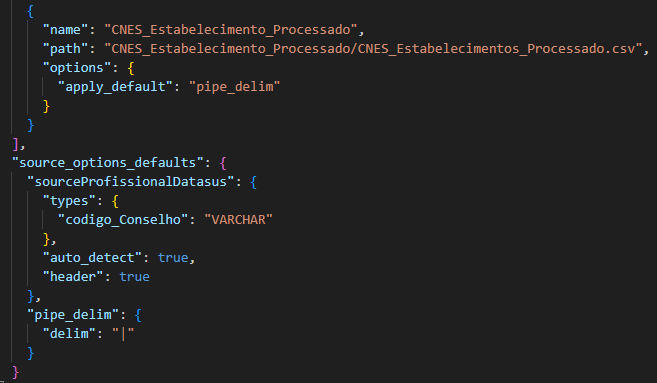
\includegraphics[width=.6\linewidth]{imagens/json.png}
  \par
  \footnotesize{Fonte: Documentos da empresa.}
\end{figure}

\subsection{Git/Github}

Git é um sistema de controle de versão distribuído que permite aos desenvolvedores rastrear mudanças no código-fonte, colaborar de forma eficiente e gerenciar o histórico do projeto com precisão. Ele suporta funcionalidades de ramificação (branching), fusão (merging) e reversão (rollback), que são essenciais para manter fluxos de trabalho de desenvolvimento limpos e organizados, especialmente em ambientes com múltiplos desenvolvedores.\cite{git_docs}

GitHub é uma plataforma de hospedagem baseada na web para controle de versão usando Git, que oferece ferramentas para rastreamento de issues, gerenciamento de projetos e automação de fluxos de trabalho através do GitHub Actions. Ele facilita a colaboração entre desenvolvedores por meio de pull requests, revisões de código e discussões, promovendo um desenvolvimento mais transparente e participativo. A utilização do GitHub é central para a gestão de código-fonte, especialmente em projetos de código aberto, simplificando os processos de integração e entrega contínua (CI/CD).\cite{github_home}

\subsection{Azure Storage Explorer}

  O Azure Storage Explorer é uma aplicação de desktop gratuita da Microsoft que fornece uma interface gráfica (GUI) para gerenciar facilmente os recursos de armazenamento do Azure. Ele funciona em Windows, macOS e Linux, permitindo que desenvolvedores, administradores de nuvem e profissionais de TI interajam com suas contas de armazenamento sem precisar escrever código ou usar linhas de comando.\cite{microsoft_azure_storage}

\subsection{R}

R é uma linguagem e um ambiente para computação estatística e gráficos. O R oferece uma ampla variedade de técnicas estatísticas (modelagem linear e não linear, testes estatísticos clássicos, análise de séries temporais, classificação, clusterização, etc.) e gráficas, e é altamente extensível. Um dos pontos fortes do R é a facilidade com que gráficos de alta qualidade, prontos para publicação, podem ser produzidos, incluindo símbolos e fórmulas matemáticas quando necessário.\cite{r_project_about}

\subsection{SQL}

A Linguagem de consulta estruturada (SQL) é uma linguagem de programação para armazenar e processar informações em um banco de dados relacional. Um banco de dados relacional armazena informações em formato tabular, com linhas e colunas representando diferentes atributos de dados e as várias relações entre os valores dos dados. Você pode usar instruções SQL para armazenar, atualizar, remover, pesquisar e recuperar informações do banco de dados. Também pode usar SQL para manter e otimizar a performance do banco de dados.\cite{aws_what_is_sql}

\subsection{YAML}

O YAML é uma linguagem legível de serialização de dados muito usada na escrita de arquivos de configuração. Dependendo, a sigla YAML pode significar em inglês "Yet Another Markup Language" (mais uma linguagem de marcação) ou "YAML Ain’t Markup Language" (YAML não é linguagem de marcação) [acrônimo recorrente]. Ambos destacam que o YAML é voltado para os dados, e não documentos. 

YAML é uma linguagem de programação famosa porque foi desenvolvida para ser fácil de ler e entender. Ele também pode ser utilizado com outras linguagens de programação.\cite{redhat_what_is_yaml}

\begin{figure}[H]
  \centering
  \caption{Exemplo de formato YAML}\label{fig:yaml}
  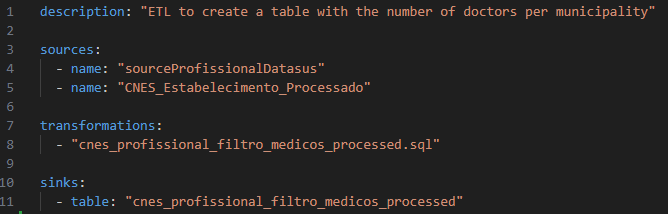
\includegraphics[width=.6\linewidth]{imagens/yaml.png}
  \par
  \footnotesize{Fonte: Documentos da empresa.}
\end{figure}

\chapter{Capítulo 4}

Requisitos gerais,  funcionais  e  não  funcionais, a  serem  cumpridos com  o  que  se  propõe desenvolver,  descrição  *conceitual*  do  que fizeram,    do  novo  jeito  de  funcionar,  fluxos  de informação e materiais, diagramas, etc., deixando claro em que medida essas coisas resolvem o problema  que  se  deseja,  as  decisões  que  foram  toma das  e  o  porquê  /  embasamento  dessas decisões, e alinhamento disso àqueles requisitos.

Deve-se fazer uma descrição “conceitual” do que fizeram, da nova maneira de funcionar, fluxos de informação e materiais, diagramas, modelos, arquiteturas, etc., deixando claro em que medida o que e forma como projetaram / idealizaram atacam o problema identificado na Introdução. 
Aqui também deve ser colocada a Metodologia usada (não confundir isso com a lista das fases do cronograma), no sentido de “como” (o raciocínio lógico, os modelos dos quais se buscou o embasamento teórico, etc.) e com base no que propuseram a proposta.
Pode, também, ser dividido em mais de um capítulo se for o caso.

\chapter{Capítulo 5}

Para solucionar o problema da complexidade e descentralização dos dados, foi projetada e desenvolvida uma arquitetura de software robusta, focada em automação, modularidade e escalabilidade. Este capítulo descreve conceitualmente a solução implementada, detalhando o fluxo de dados, a arquitetura do sistema e os componentes de software que o compõem. A metodologia adotada buscou o desacoplamento de responsabilidades e a configuração declarativa, permitindo que o sistema seja flexível e de fácil manutenção.

\section{Arquitetura geral e fluxo de dados}

A solução opera em um sistema de processamentos de dados em lote. O fluxo de informações foi desenhado seguindo um modelo de sepração entre camadas, conforme ilustrado na Figura \ref{fig:diagrama} e descritos nos passos abaixos: 

\begin{figure}[H]
  \centering
  \caption{Diagrama do projeto}\label{fig:diagrama}
  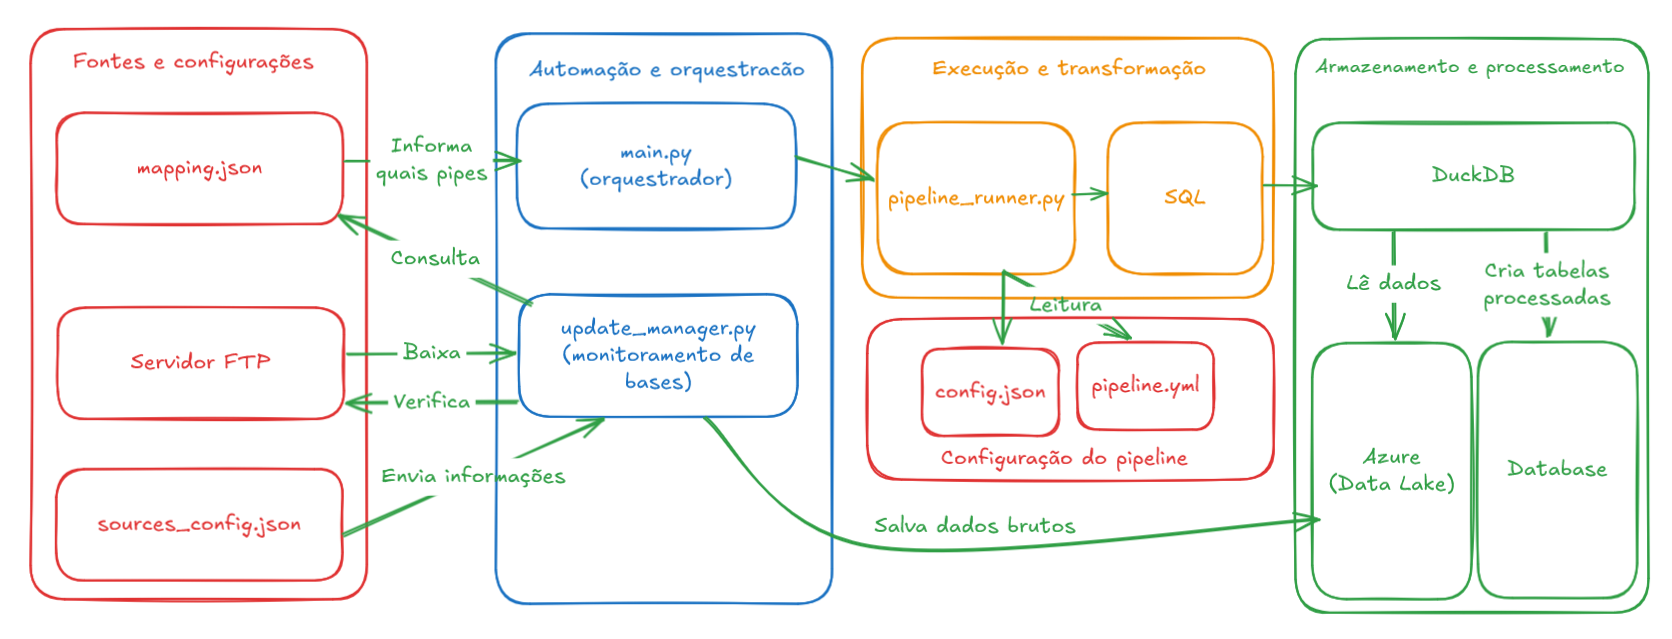
\includegraphics[width=1\linewidth]{imagens/diagrama.png}
  \par
  \footnotesize{Fonte: Documentos da empresa.}
\end{figure}

\subsection{Fontes e configurações}

A parte inicial do sistema são as fontes de dados externa, que são acessadas através dos servidores FTP do DATASUS e da ANS, onde são disponibilizados os arquivos públicos.

Os arquivos de configuração, acessados pelos orquestradores, contém informações essenciais para o pipeline. Através do $sources\_config.json$, obtemos todos os detalhes principais de cada fonte, e última vez que atualizamos esta base de dados. O $mapping.json$ é encarregado de informar quais fontes cada pipeline utiliza, para que possamos processar apenas os que tiveram uma fonte atualizada.

\subsection{Automação e orquestração}

Foi configurado para que o ciclo de processamento seja iniciado de forma autônoma duas vezes por més através do $update\_manager.py$, o agente que monitora continuamente as fontes de dados. Ao detectar um arquivo novo, é verificado quais pipelines serão processados, e em seguida realizado a chamada do $main.py$ para executar o orquestramento de cada um.

\subsection{Configuração do pipeline}

Cada pipeline é definido com um conjunto de arquivos de configuração. O $pipeline.yml$ atua como uma receita, onde especifica quais fontes devem ser lidas, a sequências de transformações em SQL a serem aplicadas e as tabelas finais a serem salvas.
Enquanto o  $config.json$, detalha os aspectos técnicos de cada fonte, como o caminho bruto no Azure, delimitador e codificação de caracteres.

\subsection{Execução e transformação}

Quando iniciado, o $pipeline\_runner.py$ assume a execução. Através do DuckDB, ele é reponsável por ler os dados diretamente da camada bruta do Azure, a lógica da transformação contida nos scripts SQL, e então, executada em memória. Esta fase é a responsável pela limpeza, padronização, junção e enriquecimento dos dados.

\subsection{Armazenamento e processamento}

O motor de processamento é o DuckDB, escolhido pela alta performance em cargas grandes de trabalho. O armazenamento é gerenciado pelo Azure Blob Stora, que funciona como um Data Warehouse. No final do fluxo, os dados processados são carregados para o Azure, onde ficam disponívems em um formato otimizado para consumo por aplicações analíticas e pela plataforma de inteligência de mercado da LifesHub.
\chapter{Capítulo 6}

Análise  dos  resultados:  análise  crítica  e  profunda  sobre  o  que fizeram,  os  resultados atingidos,  os  prós  e  contras,  impactos  da sua  utilização  na  empresa,  como  "provam"  que  isso resolveu  (ou  melhorou)  o  problema  inicialmente  identificado,  os  indicadores usados  para avaliação (e o porquê deles e não outros), os ganhos quanti ou qualitativos obtidos, etc..


Onde se apresentam e são discutidos os resultados (simulados, piloto ou reais) obtidos no decorrer da pesquisa/desenvolvimento. 
Nesta discussão é importante dar meios para que o leitor entenda os resultados obtidos e como foram obtidos.
Deve-se fazer uma análise dos resultados: análise crítica profunda sobre o que foi feito, os resultados atingidos, os prós e contras, impactos, como isso resolveu o problema, os ganhos obtidos, etc.
\chapter{Capítulo 7}

Conclusões gerais: "resumão" do que foi feito e dos resultados globais, limitações do que foi desenvolvido e pressupostos assumidos, e sugestão para trabalhos futuros de continuação.

Síntese pessoal, objetiva, sucinta e interpretada dos resultados do trabalho.
Grosso modo, deve-se apresentar um resumo do que foi feito, dos resultados globais (frente aos objetivos inicialmente traçados). Exemplos:

\begin{itemize}
\item o método deu certo? funcionou? deu o resultado esperado? Foi melhor que o método anterior?
\item impactos organizacionais, tecnológicos, financeiros, éticos, ecológicos, etc., tidos (ou potencialmente a ter) com a introdução do que foi proposto.
\end{itemize}


De forma complementar, se pertinente, sugestões para trabalhos futuros de continuação.

% ----------------------------------------------------------
% Finaliza a parte no bookmark do PDF
% para que se inicie o bookmark na raiz
% e adiciona espaço de parte no Sumário
% ----------------------------------------------------------
\phantompart

% ----------------------------------------------------------
% ELEMENTOS PÓS-TEXTUAIS
% ----------------------------------------------------------
\postextual
% ----------------------------------------------------------

% ----------------------------------------------------------
% Referências bibliográficas
% ----------------------------------------------------------

\bibliography{bibliografia}

% ----------------------------------------------------------
% Apêndices
% ----------------------------------------------------------

% ---
% Inicia os apêndices
% ---
\begin{apendicesenv}

\chapter{Título Opcional}
Textos elaborados pelo próprio autor, a fim de complementar a sua argumentação

\end{apendicesenv}
% ---


% ----------------------------------------------------------
% Anexos
% ----------------------------------------------------------

% ---
% Inicia os anexos
% ---
\begin{anexosenv}

% ---
\chapter{Título Opcional.}
% ---
Documentos não elaborados pelo autor, utilizados de fundamentação (mapas, leis, estatutos).

\end{anexosenv}

%---------------------------------------------------------------------
% INDICE REMISSIVO
%---------------------------------------------------------------------
\phantompart
\printindex
%---------------------------------------------------------------------

\end{document}
